%!TEX root = ../Dimensionieren I.tex

\section{Normalspannungshypothese (Rankine)} % (fold)
	\textbf{Annahme:} Versagen durch Trennbruch senkrecht zur grössten Normalspannung ($\sigma_1$) durch \textbf{sprödes Materialverhalten}, \emph{zweiachsiger Spannungszustand} ($\sigma_Z = 0$).
	
	\textbf{Vergleichsspannung:}
	\begin{equation*}
		\sigma_V = \sigma_1= \frac{\sigma_x + \sigma_y}{2} + \frac{1}{2} \sqrt{(\sigma_x - \sigma_y)^2 + 4 \tau_{xy}^2}
	\end{equation*}
% section: Normalspannungshypothese (end)
\section{Schubspannungshypothese (Tresca)} % (fold)
	\textbf{Annahme:} Versagen durch Fliessen (\textbf{zähes Materialverhalten}).
	
	\textbf{Vergleichsspannung:}
	\begin{align*}
		\sigma_V &= 2 \tau_{\text{max}} = \sigma_{\text{max}}-\sigma_{\text{min}} = \sigma_1 - \sigma_3 \\
		\sigma_3 &= 0: \quad \sigma_V = \frac{1}{2} (\sigma_x - \sigma_y) + \frac{1}{2}\sqrt{(\sigma_x-\sigma_y)^2 + 4 \tau_{xy}^2} \\
		\sigma_2 &= 0: \quad \sigma_V = \sqrt{(\sigma_x - \sigma_y)^2 + 4 \tau_{xy}^2}
	\end{align*}
% section: Schubspannungshypothese (Tresca) (end)
\section{Gestaltänderungshypothese (Mises)} % (fold)
	\textbf{Annahme:} Fliessen tritt erst ein, wenn die für die Gestaltänderung notwendigen Arbeiten beim mehrachsigen und einachsigen Spannungszustand gleich sind.
	
	\textbf{Dreiachsiger Spannungszustand:}
	{\setlength{\mathindent}{0pt}
	\begin{align*}
		\sigma_V &= \sqrt\frac{(\sigma_x - \sigma_y)^2 + (\sigma_y - \sigma_z)^2 + (\sigma_z - \sigma_x)^2 + 6(\tau_{xy}^2 + \tau_{yz}^2 + \tau_{zy}^2)}{2} \\
		\sigma_V &= \sqrt\frac{(\sigma_1 - \sigma_2)^2 + (\sigma_2 - \sigma_3)^2 + (\sigma_3 - \sigma_1)^2}{2} 
	\end{align*}}
	
	\textbf{Zweiachsiger Spannungszustand:}
	\begin{equation*}
		\sigma_V = \sqrt{\sigma_x^2 + \sigma_y^2 - \sigma_x\sigma_y + 3 \tau_{xy}^2}
	\end{equation*}
% section: Gestaltänderungshypothese (von Mises) (end)
\section{Zulässige Vergleichsspannung} % (fold)
	\begin{equation*}
		\sigma_{\text{zul}} = \underbrace{\frac{\sigma_F}{S_F}}_{\text{Fliessen}} = \underbrace{\frac{\sigma_B}{S_B}}_{\text{Bruch}}
	\end{equation*}
	mit $S_F \in [1.2 , 2.0]$ und $S_B \in [2 , 4]$.

	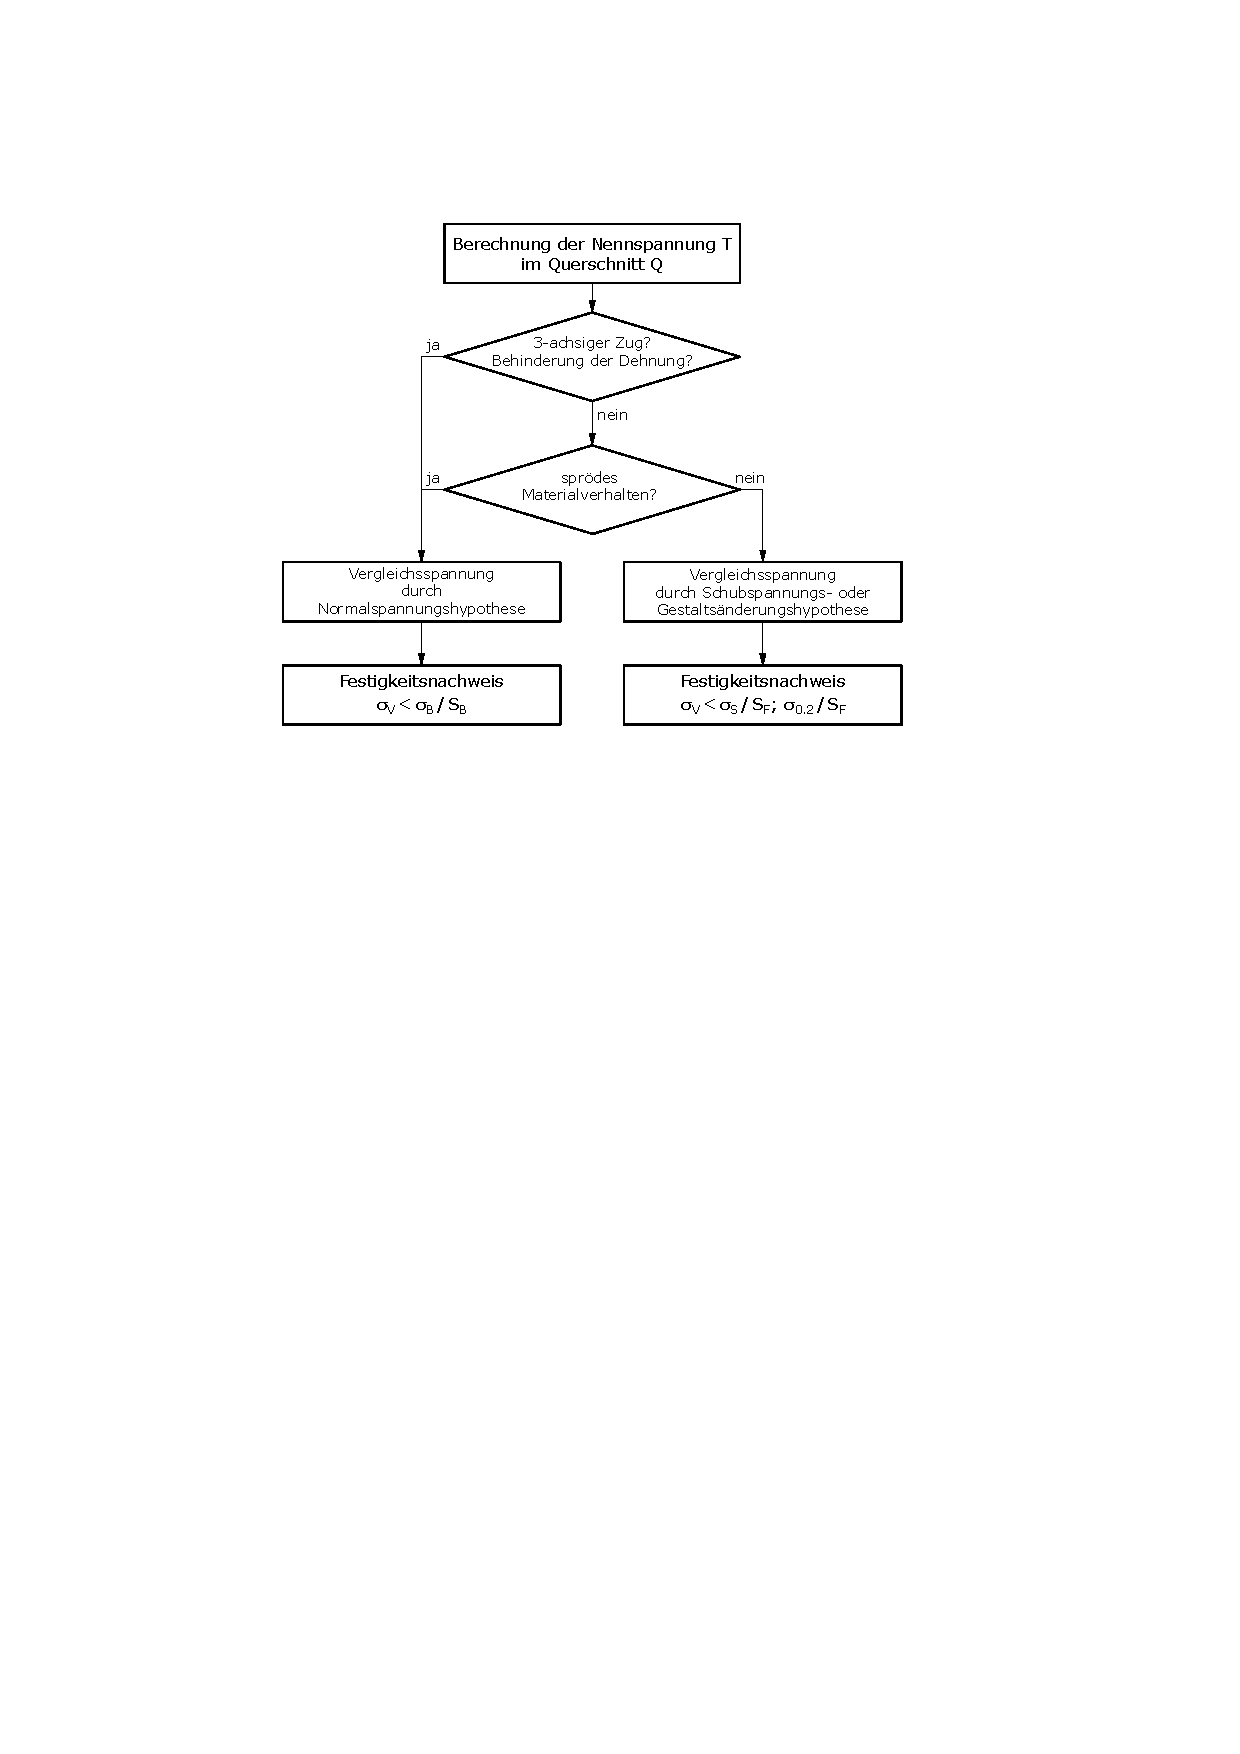
\includegraphics[width=\columnwidth]{graphics/abb_3_10}
	
	Bauteilfliessgrenze (vereinfacht):
	\begin{equation*}
		\sigma_\text{bFK} = K_1(d)\cdot \sigma_S(d_B)
	\end{equation*}
% section: Zulässige Vergleichsspannung (end)
\section{Bauteilbeanspruchung oberhalb Grenzbeanspruchung} % (fold)
	\subsection{Plastische Reserve} % (fold)
		Bedingungen:
		\begin{tightitemize}
			\item Zähes Materialverhalten, existente Reserve
			\item Gute Berechnungsgrundlage
			\item Deformation ohne Einfluss auf Funktion
			\item Keine gesetzlichen Vorgaben
			\item Folgen des Versagens abschätz- und verantwortbar
		\end{tightitemize}
	% subsection: Plastische Reserve (end)
	\subsection{Beanspruchungsbedingte Reserve} % (fold)
		Nur Teile des Querschnitts werden oberhalb Grenzbeanspruchung beansprucht. Zum Beispiel Biegestab, Kerben, durckbelastete, rotationssymmetrische Bauteile, etc.
	% subsection: Beanspruchungsbedingte Reserve (end)
	\subsection{Bruch} % (fold)
		Im Falle des Bruchs gilt: $S_B = 1$
	% subsection: Bruch (end)
% section: Bauteilbeanspruchung oberhalb Grenzbeanspruchung (end)